%-----------------------------------------------------------------------------%
\chapter{\babEmpat}
\label{chap:babEmpat}
%-----------------------------------------------------------------------------%

Pada bab ini dijelaskan hasil evaluasi dan analisis dari penelitian ini.

%-----------------------------------------------------------------------------%
\section{Evaluasi}
%-----------------------------------------------------------------------------%

Dua eksperimen pada penelitian ini dilakukan pada \textit{notebook} dengan sistem operasi \textit{Ubuntu 15.04 64-bit}, prosesor \textit{Intel Core i7 5500U} (\textit{dual cores}), RAM DDR3 8 GB dan penyimpanan SSD 250 GB. Program yang digunakan untuk melakukan eksperimen pertama adalah \verb|classifier.py| sedangkan eksperimen yang kedua menggunakan program \verb|extract_triples.py| (terlampir).

Pada eksperimen pertama, empat model \textit{supervised learning} dilatih dan diuji menggunakan data kandidat \textit{triple} yang sudah diberikan label, diekstraksi menjadi 17 fitur dan dinormalisasi. Metode yang digunakan untuk melatih dan menguji adalah \textit{k-fold} \textit{cross-validation} \citep{kohavi1995study} dengan $k = 3$. Empat model yang dibandingkan beserta dengan konfigurasinya adalah sebagai berikut:

\begin{enumerate}

	\item Linear Logistic Regression
	\begin{itemize}
		\item Solver (cost function): \verb|liblinear|
		\item Penalty (regularizer): \verb|l2|
	\end{itemize}

	\item Polynomial Support Vector Machine (SVM)
	\begin{itemize}
		\item Kernel: \verb|poly|
		\item Degree: \verb|5|
	\end{itemize}

	\item ReLU Multi-Layer Perceptron (MLP)
	\begin{itemize}
		\item Hidden layers: \verb|(20, 10)|
		\item Activation: \verb|relu| \citep{nair2010rectified}
		\item Max. iteration: \verb|1000|
	\end{itemize}
	
	\item Random Forest
	\begin{itemize}
		\item Max. depth: \verb|8|
		\item Number of estimators: \verb|20|
		\item Min. samples split: \verb|5|
		\item Criterion: \verb|gini| \citep{mingers1989empirical}
		\item Max. features: \verb|auto| (pembulatan akar dari jumlah total fitur)
		\item Class weight: \verb|balanced| (sesuai rasio kelas)
	\end{itemize}

\end{enumerate}

Eksperimen ini dilakukan dengan menjalankan program \verb|classifier.py| (di direktori yang sama dengan pustaka utama \verb|tripletools.py|) dengan input data fitur yang sudah dinormalisasi dengan format \textit{comma separated value} (CSV) \verb|triple-selector.train.csv| pada \textit{terminal}:

\begin{verbatim}
	$ python classifier.py --best triple-selector.train.csv
\end{verbatim}

Hasil dari eksperimen pertama ini dapat dilihat pada Tabel \ref{tab:models_performance} dan visualisasinya pada Gambar \ref{fig:models_performance} di mana \textit{random forest} mencapai nilai \textit{recall} dan $F_1$ tertinggi, yaitu \textbf{0.58}. Sedangkan nilai \textit{precision} tertinggi, \textbf{0.68}, dicapai oleh SVM. 

\begin{figure}
	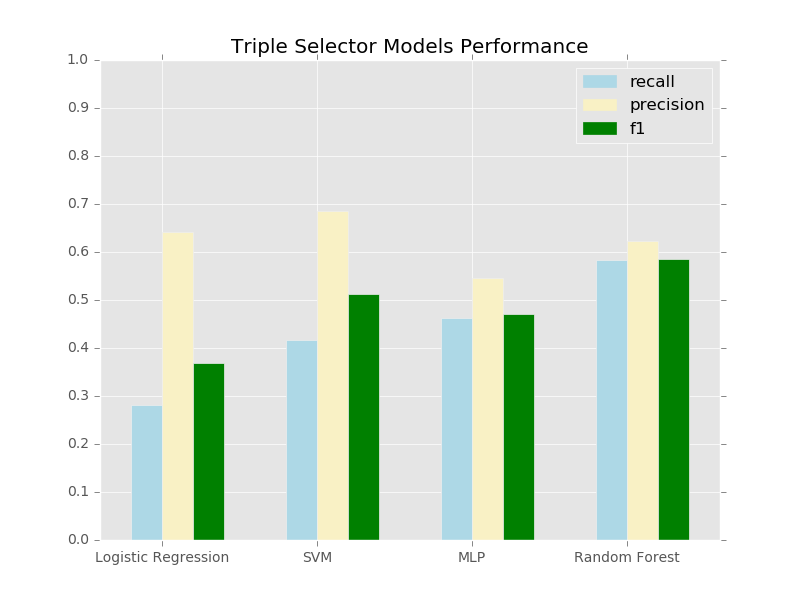
\includegraphics[width=\textwidth]{../images/models_performance.png}
	\caption{Diagram hasil eksperimen perbandingan model \textit{supervised learning} untuk \textit{triple selector}}
	\label{fig:models_performance}
\end{figure}

\begin{table}
\caption{Hasil eksperimen perbandingan model \textit{supervised learning} untuk \textit{triple selector}}
	\label{tab:models_performance}
	\centering
	\begin{tabular}{p{5cm} >{\centering\arraybackslash}p{2cm} >{\centering\arraybackslash}p{2cm} >{\centering\arraybackslash}p{2cm}}
		\hline
		\textbf{Model} & \textbf{\textit{Precision}} & \textbf{\textit{Recall}} & \textbf{$F_1$} \\
		\hline
		Logistic Regression & 0.64 & 0.28 & 0.36 \\
		SVM & \textbf{0.68} & 0.41 & 0.51 \\
		MLP & 0.54 & 0.46 & 0.47 \\
		Random Forest & 0.62 & \textbf{0.58} & \textbf{0.58} \\
		\hline
	\end{tabular}
\end{table}

Pada eksperimen kedua, sistem \textit{open IE} dipakai untuk mengekstrak \textit{triple} dari tiga buah dokumen dengan ukuran bervariasi. Metrik utama pada eksperimen ini adalah waktu total eksekusi yang dipakai untuk menghitung waktu eksekusi rata-rata per kalimat. Sebagai tambahan, diamati juga jumlah \textit{triple} yang dapat diekstraksi dari tiap dokumen. Eksperimen ini dilakukan dengan menjalankan program utama \verb|extract_triples.py| untuk setiap dokumen (\verb|doc1.txt|, \verb|doc2.txt|, \verb|doc3.txt|) yang berisi satu kalimat per baris:

\begin{verbatim}
	$ python extract_triples.py -f tsv doc1.txt
	$ python extract_triples.py -f tsv doc2.txt
	$ python extract_triples.py -f tsv doc3.txt
\end{verbatim}

Hasil eksperimen tersebut ditunjukkan pada Tabel \ref{tab:system_extraction_time} di mana waktu eksekusi rata-rata per kalimat \textbf{0.014 detik/kalimat} dicapai untuk ukuran dokumen terbesar 5,593 kalimat. Dapat dilihat bahwa rata-rata waktu yang dibutuhkan untuk memproses satu kalimat semakin menurun seiring dengan bertambahnya jumlah kalimat pada dokumen. Rata-rata jumlah \textit{triple} yang diekstraksi dari setiap dokumen adalah \textbf{3.3 \textit{triple}/kalimat}.

\begin{table}
	\caption{Waktu eksekusi sistem \textit{open IE} \textit{end-to-end}}
	\label{tab:system_extraction_time}
	\centering
	\begin{tabular}{p{4cm} p{2.5cm} p{2.5cm} p{2.5cm}}
		\hline
		\textbf{Jumlah kalimat} & \textbf{\textit{Triple}} & \textbf{Total (detik)} & \textbf{Per kalimat (detik)} \\
		\hline
		2 & 7 & 6.1 & 0.800 \\
		138 & 429 & 11.3 & 0.082 \\
		5,593 & 19,403 & 78.6 & 0.014 \\
		\hline
	\end{tabular}
\end{table}

%-----------------------------------------------------------------------------%
\section{Analisis}
%-----------------------------------------------------------------------------%

The first experiment shows that all classifiers are still having problem learning the pattern of triples when cross-validated using $k=3$ which means two thirds of our dataset is insufficient to cover the patterns in other one third part. The dataset also suffers unbalance 1:11 ratio of positive and negative samples which is caused by lack of efficiency in triple candidates generator. To solve this issue, we plan to annotate more sentences to increase the coverage and improve the efficiency of triple candidates generator. The low performance of linear logistic regression indicates that this problem is not linearly separable. The random forest performs better than other nonlinear models (SVM and MLP) because it is easily tuned to balance the precision and recall by changing the number and the depth of decision trees.

We are also aware that the heuristics used in triple candidates generator and token expander are still limited to explicit pattern. For instance, triple candidate generator can not extract relations \textit{(kecamatan Kejajar, terletak di, Jawa Tengah)} and \textit{(Jawa Tengah, terletak di, Indonesia)} from the sentence in Figure \ref{fig:example_io_openie} yet. In the future research, we plan to improve the model to extract implicit patterns while keeping the number of negative candidates. The token expander is having problem in expanding token to implicitly expected clauses such as \textit{"seorang pelatih sepak bola"} from \textit{"seorang pelatih dan pemain sepak bola"} or \textit{"satu buah torpedo"} from \textit{"satu atau dua buah torpedo"}. We expect there will be more patterns that need to be considered in order to properly expand the token so further research on effective model to achieve this is required. Also, in order to properly evaluate the performance of these components, we need to create test datasets for both triple candidates generator and token expander.

Additionally, through the second experiment, we also find that our system average extraction performance is 0.014 seconds/sentence (for 5,593 sentences document) which is still comparable to TextRunner\citep{banko2007open}. Therefore, in contrast to the argument proposed in the related work\citep{banko2007open}\citep{etzioni2011open}, this experiment shows that the heavy linguistic tasks such as dependency parsing doesn't cause performance drawback in big document, assuming the average number of sentences in document do not exceed 5,593.
